\documentclass[light]{lutbeamer} % change between light and dark for the background
%\documentclass[t]{lutbeamer} % use "t" option for top alignment 

\usepackage{pgfpages}
\setbeameroption{hide notes} % Only slides
% \setbeameroption{show only notes} % Only notes
% \setbeameroption{show notes on second screen=right} % Both

\setdepartment{INRAE}
\institute[M2P2 team]{Institut national de la recherche agronomique}
\author{Taha Belkhayate}
\title[Drosophila suzukii]{drosophila suzukii's (SWD) overview}
\subtitle{Mathematical Modeling}
\date{\today}


\begin{document}

% front page
{ % all template changes are local to this group.
    \setbeamertemplate{navigation symbols}{}
    \begin{frame}<article:0>[plain,noframenumbering]
        \begin{tikzpicture}[remember picture,overlay]
            \node[at=(current page.center)] {
                \includegraphics[
                                 width=\paperwidth,
                                 height=\paperheight]{logos/front}
            };
        \end{tikzpicture}
    \end{frame}
}

% Outline
\AtBeginSection[]
{
\begin{frame}[plain,noframenumbering]
\frametitle{Outline}
\begin{columns}[T]
    \begin{column}{0.01\textwidth}
        
    \end{column}
    \begin{column}{0.95\textwidth}
        \tableofcontents[currentsection,
                        %currentsubsection,
                        %hideothersubsections, 
                        %sectionstyle=show/shaded, 
                        %subsectionstyle=show/shaded%/hide
                 ]
    \end{column}
\end{columns}
\end{frame}
}


% use blurred background figure
% {\usebackgroundtemplate{%
% \begin{tikzpicture}[remember picture,overlay]
% \node [anchor=south east, 
%       xshift=2.15cm, 
%       yshift=0.25cm,
%       opacity=0.35, scale=0.3]  at (current page.south east)  {\includegraphics{figures/figurename}};
% \end{tikzpicture}
% }
{ % title page
\begin{frame}[plain]
\maketitle
\small
\par\vskip0.5em
{\footnotesize
    \hspace*{0.2cm}
    \begin{tabular}[t]{@{}l@{\hspace{4pt}}p{.5\textwidth}@{}}
    Supervisors: & VAN OUDENHOVE Louise, COURTOIS Marine, Ludovic Mailleret
    \end{tabular}%
    \par\vskip0.5em
    \hspace*{0.26cm}\begin{tabular}[t]{@{}l@{\hspace{3pt}}p{.5\textwidth}@{}}
    %Opponent: & Prof. Opponent, University
    \end{tabular}%
    }
\note[item]{
Honored custos, honored opponent, honored listeners, ...
}
\end{frame}
}

\section{Introduction}
\subsection{THE INVASIVE SPECIES}
\begin{frame}
\frametitle{The invasive species}
\framesubtitle{}
\begin{itemize}
\item Drosophila suzukii is considered an r-strategist species
%\hrefcol{http://en.wikibooks.org/wiki/LaTeX/}{you can learn it here}

%Beamer is one of the most popular and powerful document classes for presentations in \LaTeX
\item Drosophila suzukii exhibits a lek mating system
%\hrefcol{http://www.ctan.org/tex-archive/macros/latex/contrib/beamer/doc/beameruserguide.pdf}{user manual}
\item High rate of ovipostion.
\end{itemize}
\end{frame}

\begin{frame}
\subsection{ECONOMIC IMPACT OF DROSOPHILA SUZUKII}
\frametitle{Economic impact of drosophila suzukii}

\begin{itemize}
\item \textbf{The economic impact of Drosophila suzukii: perceived costs and revenue losses of Swiss cherry, plum and grape growers (2020)}
\item the study estimates the overall economic impact of Drosophila suzukii on the Swiss fruit industry to be around CHF 13 million (approx. USD 14.3 million) per year $\eq$ 13 millions euro
\item \textbf{Recent Trends in the Economic Impact of Drosophila suzukii}
\item In the United States, estimated losses due to D. suzukii infestation ranged from USD 511 million to USD 2.6 billion in 2010-2016.
In Europe, the economic impact of D. suzukii varied depending on the crop and region. For example, in Italy, losses in cherry production ranged from 13\% to 80\%.
In Asia, D. suzukii has been a significant pest of raspberry and blueberry crops, causing up to 100\% yield losses in some cases.
%\item Produces side notes
%\item Math typesetting in \TeX\ is the best:
%\begin{equation*}
%\mathrm{i}\,\hslash\frac{\partial}{\partial t} \Psi(\mathbf{r},t) =
%-\frac{\hslash^2}{2\,m}\nabla^2\Psi(\mathbf{r},t)
%+ V(\mathbf{r})\Psi(\mathbf{r},t)
%\end{equation*}

\end{itemize}
\end{frame}

\subsection{Drosophila suzukii's characteristics}
\begin{frame}
\frametitle{The female's characteristic}
\framesubtitle{}
\begin{itemize}
\item high reproductive rate and a short generation time,
%\hrefcol{http://en.wikibooks.org/wiki/LaTeX/}{you can learn it here}
%Beamer is one of the most popular and powerful document classes for presentations in \LaTeX
\item females mated on average twice with an average of 16 days between each mating. (Debatable)
\item females more resistant to cold than males
\item A winter with several days of intense cold causes high mortality in the population especially.
\item spring, females are always more numerous than males
\item summer: the proportion of males and females is then balanced 
\item The sex ratio of newly emerged adults is on average 1
%\hrefcol{http://www.ctan.org/tex-archive/macros/latex/contrib/beamer/doc/beameruserguide.pdf}{user manual}

\end{itemize}
\end{frame}

\begin{frame}
\frametitle{The male's characteristic}
\framesubtitle{}
\begin{itemize}
%Sexual Behavior of Drosophila suzukii
%Santosh Revadi,1 Sébastien Lebreton,1 Peter Witzgall,1 Gianfranco Anfora,2 Teun Dekker,1 and Paul G. Becher1,* (2015)
\item high reproductive rate and a short generation time,
%\hrefcol{http://en.wikibooks.org/wiki/LaTeX/}{you can learn it here}%Beamer is one of the most popular and powerful document classes for presentations in \LaTeX
\item autumn: finally reversed males more than females
\item males more resistant to heat than females
\item In some cases, males may exhibit aggressive behavior towards each other as they compete for access to females. 
\item autumn: finally reversed males more than females
\item have a high re-mating rate and can mate multiple times in a day. In laboratory studies, males have been observed to mate up to 20 times in a 24-hour period. 
%\hrefcol{http://www.ctan.org/tex-archive/macros/latex/contrib/beamer/doc/beameruserguide.pdf}{user manual}

\end{itemize}
\end{frame}


%\begin{frame}[fragile]
%\frametitle{Selecting the Class}
%To start working with \texttt{lutbeamer}, start a \LaTeX\ document with the
%preamble:
%\begin{block}{Minimum LUT Beamer Document}
%\verb|\documentclass[light]{lutbeamer} % or [dark]|\\
%\verb|\setbeameroption{hide notes} % or {show only notes} or| 
%\verb|% {show notes on second screen=right}|\\
%\verb|\begin{document}|\\
%\verb|\begin{frame}{Hello, world!}|\\
%\verb|\framesubtitle{Subtitle}|\\
%\verb|\end{frame}|\\
%\verb|\end{document}|\\
%\end{block}
%\end{frame}

%\begin{frame}[fragile]
%\frametitle{Title page}
%To set a typical title page, you call some commands in the preamble:
%\begin{block}{The Commands for the Title Page}
%\begin{verbatim}
%\setdepartment{LUT School of ... }
%\author{Author}
%\title[Short presentation title]{Presentation title}
%\subtitle{Presentation subtitle}
%\date{Defaults to today's}
%\end{verbatim}
%\end{block}
%\end{frame}

\subsection{Mathematical model}

\begin{frame}[fragile]
\frametitle{Mathematical model}
\framesubtitle{With and Without the release of sterile species}
\begin{itemize}[<+->]
\only<1-3>{\item without the release we have 
$$\left\{\begin{array}{l}\frac{d L}{d t}=\beta\left(1-\frac{L}{K}\right) F-\left(v_L+\mu_L\right) L \\ \frac{d M}{d t}=v_L m L-\mu_M M \\ \frac{d V}{d t}=v_L(1-m) L-\mu_F V-v_F \min \left(\frac{M}{V}, 1\right) V \\ \frac{d F}{d t}=v_F \min \left(\frac{M}{V}, 1\right) V-(\mu_F+\gamma) F\end{array}\right.$$

\item 
$$\left\{\begin{array}{l}\frac{d L}{d t}=\beta\left(1-\frac{L}{K}\right) F-\left(v_L+\mu_L\right) L \\ \frac{d M}{d t}=v_L m L-\mu_M M \\ \frac{d V}{d t}=v_L(1-m) L-\mu_F V-v_F \min \left(\frac{M}{\gamma F+V}, 1\right) V \\ \frac{d F}{d t}=v_F \min \left(\frac{M}{V+ \gamma F}, 1\right) V-\mu_F F\end{array}\right.$$

\item $$\left\{\begin{array}{l}\frac{d L}{d t}=\beta\left(1-\frac{L}{K}\right)v_F \min \left(\frac{M}{\gamma F + V}, 1\right) F-\left(v_L+\mu_L\right) L \\ \frac{d M}{d t}=v_L m L-\mu_M M \\ \frac{d F}{d t}=v_L(1-m) L-\mu_F F \end{array}\right.$$}%\includegraphics[width=\textwidth]{female.png}


\only<5-5>{\item with the release of both sexes \begin{figure}[h!]
\includegraphics[width=11cm]{female.png}
\end{figure}}

\only<6-6>{\item {$$\left\{\begin{array}{l}
\dot{L} =\beta\left(1-\frac{L}{K}\right) F-\left(\mu_L+v_L\right) L \\ \dot{V}=v_L(1-m) L +\delta F + \gamma V_s-(\mu_V + v_v(P_{VM} +P_{VM_s}))V  \\\dot{V_s}=v_vP_{VM_s}V-(\mu_V+\gamma)V_s  \\  \dot{F}= v_vP_{VM} V-(\mu_F+\delta) F  \\  \dot{M} =v_L m L-\mu_M M \\ \dot{M_s} =\phi_1 (t)-\mu_M_s M_s \\ \dot{F_s} =\phi_2 (t)-\mu_{F_s} F_s
\end{array}\right.$$}
% By separating the contributions of wild and sterile males and females to the probability of successful mating, you are implicitly assuming that the attraction and courtship behaviors of wild and sterile individuals are independent and that the presence of sterile individuals does not interfere with the ability of wild males and females to find and court each other.
%\item $$P(FM|FX)=\frac{P(FM \cap FX)}{P(FX)}=\frac{P_{FM}}{P_{FM}+P_{FM_s}}$$

\item $$P_{VM}=\frac{\beta_{VM}M \beta_{MV}V}{\beta_{VM}M\beta_{MV}V+\beta_{VM_s}M_s\beta_{M_sV}V+\beta_{F_sM}M\beta_{MF_s}F_s+\beta_{F_sM_s}M_s\beta_{M_sF_s}F_s} $$

\item $$M_s(t)=e^{-\mu_{M_s}t}\left(M_s(0)+\int_0^t e^{\mu_{M_s} s}  \phi_1(s) d s\right) .$$
\item $$F_s(t)=e^{-\mu_{F_s}t}\left(F_s(0)+\int_0^t e^{\mu_{F_s}s}  \phi_2(s) d s\right) .$$
}
%\item $$P_{FM}+P_{FM_s}=\frac{\beta_{FM}M \beta_{MF}F+\beta_{FM_s}M_s \beta_{M_sF}F_s}{\beta_{FM}M\beta_{MF}F+\beta_{FM_s}M_s\beta_{M_sF}F+\beta_{F_sM}M\beta_{MF_s}F_s+\beta_{F_sM_s}M_s\beta_{M_sF_s}F_s} $$

%\item $$P(FM|FX)=\frac{\beta_{FM}M \beta_{MF}F}{\beta_{FM}M \beta_{MF}F+\beta_{FM_s}M_s \beta_{M_sF}F} $$}
\only<7-7>{\item \textbf{we didn't take into consideration the fact of the competitiveness of males, sperms, residual fertility, polygamy immigration and emigration.
\item multiple mating is not considered here because of the type of equation we are working with}}



\only<4-4> {\item {\begin{figure}[h!]
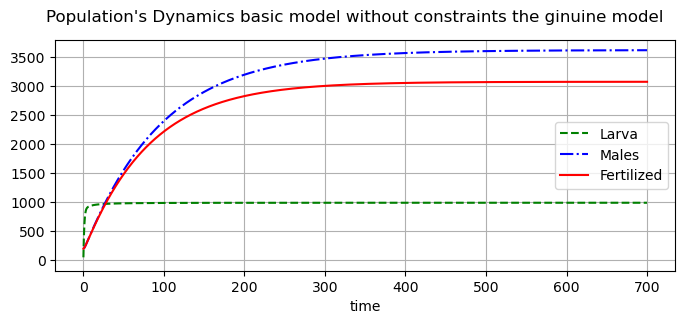
\includegraphics[width=12cm]{2.jpg}
\end{figure}}}


\end{itemize}
%\begin{block}{Code for a Page with an Itemised List}<+->
%\begin{verbatim}
%\begin{frame}
 % \frametitle{Writing a Simple Slide}
 % \framesubtitle{It's really easy!}
  %\begin{itemize}[<+->]
   % \item A typical slide has bulleted lists
    %\item These can be uncovered in sequence
  %\end{itemize}
%\end{frame}\end{verbatim}
%\end{block}
\end{frame}


\begin{frame}[fragile]
\frametitle{Critical points}
\framesubtitle{Without the release of sterile species}
\begin{itemize}[<+->]
\item without the release of sterile insects the problem is 

$$\left\{\begin{array}{l}
\dot{L} =\beta\left(1-\frac{L}{K}\right) F-\left(\mu_L+v_L\right) L \\ \dot{V}=v_L(1-m) L +\delta F-\mu_V V - v_v min(\frac{\gamma M}{V} )V\\  \dot{F}= v_v min(\frac{\gamma M}{V} )V-(\mu_F+\delta) F  \\  \dot{M} =v_L m L-\mu_M M 
\end{array}\right.$$

\item we can have two critical points at this stage the first one is $E^\# =(0,0,0,0)$ and the second is $T^\#=(L^*,V^*,F^*,M^*)$

$L^*=K-\frac{K(\mu_L+v_L)}{\beta(m-1)\mu_L}(\delta-\frac{(\mu_V+v_v)(\mu_F+\delta)}{v_v})$

$F^*=\frac{K\beta (m-1)v_Lv_v-K(v_L+\mu_L)(\delta v_v-(\mu_v + v_v)(\delta + \mu_F))}{\beta(\delta v_v-(v_v+\mu_V)(\delta + \mu_F))}$

$V^*= \frac{(\delta+\mu_F)}{v_v}F^*$ 

$M^* =\frac{v_L m}{\mu_M } L^*$

\end{itemize}

\end{frame}



\begin{frame}[fragile]
\frametitle{Mathematical model}
\framesubtitle{Realeasing only males without preferences}

\only<1-1>{$$\left\{\begin{array}{l}
\dot{L} =\beta\left(1-\frac{L}{K}\right) F-\left(\mu_L+v_L\right) L \\ \dot{V}=v_L(1-m) L +\delta F + \gamma V_s-(\mu_F+v_v) V  \\\dot{V_s}=v_vP_{VM_s}V-(\mu_F+\gamma)V_s  \\  \dot{F}= v_vP_{VM} V-(\mu_F+\delta) F  \\  \dot{M} =v_L m L-\mu_M M \\ \dot{M_s} =\phi_1 (t)-\mu_M_s M_s 
\end{array}\right.$$}
$\bullet$ critical points
\only<2-2>{$$[\eta_0 +\frac{\delta m v_L}{\mu_M\left(\mu_F+\delta\right)}-\frac{(\mu_F+v_v)v_Lm}{\mu_M v_v}]L^*-\frac{\eta_0}{K}L^{*2}=[\frac{\mu_F+v_v}{v_v}-\frac{\gamma}{\mu_F+\gamma}]M_s$$

$$F^* = \frac{\mu_L+v_L}{\beta(1-\frac{L}{K})}L^*$$

$$M^*=\frac{mv_L}{\mu_M}L^*$$

$$V^*_s=\frac{M_s(\mu_F+\delta)}{M(\mu_F+\gamma)}\frac{\mu_L+v_L}{\beta(1-\frac{L}{K})}L^*$$

$$V^*=\frac{(\mu_F+\delta)}{v_v}(1+\frac{M_s}{M})\frac{\mu_L+v_L}{\beta(1-\frac{L}{K})}L^*$$}

\only<3-3>{with  $$\eta_0=\frac{ v^2_L(1-m)m \beta}{\mu_M\left(\mu_F+\delta\right)\left(\mu_L+v_L\right)}$$}
\end{frame}

\begin{frame}[fragile]
\frametitle{Mathematical model}
\framesubtitle{Other sophisticated models, A Physiologically Based Approach}
$$
\left\{\begin{array}{c}
\frac{\partial}{\partial t} N(t, x)+\frac{\partial}{\partial x}[G(t, x) N(t, x)]=-M(t, x) N(t, x) \\
N(t, 0)=\int_0^{x_m} \beta\left(t, x^{\prime}\right) N\left(t, x^{\prime}\right) d x^{\prime} \\
N(0, x)=n^0(x)
\end{array}\right.
$$


\end{frame}

%\begin{frame}[fragile]
%\frametitle{Using Colours}
%\begin{itemize}[<alert@2>]
%  \item You can use colours with the
%        \verb|\textcolor{<color name>}{text}| command
%  \item The colours are defined in the \texttt{lutcolor} package:
%  \begin{itemize}
%  \item Primary colour: \testcolor{green};
%  \item Contrast colours: \testcolor{orange}, \testcolor{black}, \testcolor{pink};
%  \item Additional colours: \testcolor{grey}, \testcolor{gr}, 
%                            \testcolor{viridian}, \testcolor{rdbu7}
%  \end{itemize}
%  \item Do \emph{not} abuse colours: \verb|\emph{}| is usually enough
%  \item Use \verb|\alert{}| to bring the \alert<2->{focus} somewhere
%  \item<2- | alert@2> If you highlight too much, you don't highlight at all!
%\end{itemize}
%\end{frame}

%\begin{frame}[fragile]
%\frametitle{Adding images}
%\begin{columns}
%\begin{column}{0.7\textwidth}
%Adding images works like in normal \LaTeX:
%\begin{block}{Code for Adding Images}
%\begin{verbatim}
%\usepackage{graphicx}
% ...
%\includegraphics
%[width=\textwidth]{figures/Mycena_interrupta}
%\end{verbatim}
%\end{block}
%\end{column}
%\begin{column}{0.3\textwidth}
%\includegraphics
%[width=\textwidth]{figures/Mycena_interrupta}\\
%\end{column}
%\end{columns}
%\end{frame}


%\begin{frame}[fragile]
%\frametitle{Highlighting an Image region}
%\begin{center}
%\begin{tikzpicture}
%    \node[anchor=south west,inner sep=0] (image) at (0,0) {\includegraphics[width=0.6\textwidth]{figures/Mycena_interrupta.jpg}};
%    \begin{scope}[x={(image.south east)},y={(image.north west)}]
%        \draw[help lines,xstep=.1,ystep=.1] (0,0) grid (1,1);
%        \foreach \x in {0,1,...,9} { \node [anchor=north] at (\x/10,0) {0.\x}; }
%        \foreach \y in {0,1,...,9} { \node [anchor=east] at (0,\y/10) {0.\y}; }
%        \draw[red,ultra thick,rounded corners] (0.6,0.6) rectangle (0.8,0.8);
 %   \end{scope}
%\end{tikzpicture}
%\end{center}
%\end{frame}

%\begin{frame}[fragile]
%\frametitle{Splitting in Columns}
%Splitting the page is easy and common;
%typically, one side has a picture and the other text:
%\begin{columns}
%\begin{column}{0.6\textwidth}
%This is the first column
%\end{column}
%\begin{column}{0.3\textwidth}
%And this the second
%\end{column}
%\end{columns}
%\begin{block}{Column Code}
%\begin{verbatim}
%\begin{columns}
%    \begin{column}{0.6\textwidth}
 %       This is the first column
%    \end{column}
 %   \begin{column}{0.3\textwidth}
 %       And this the second
 %   \end{column}
    % There could be more!
%\end{columns}
%\end{verbatim}
%\end{block}
%\end{frame}

%\begin{frame}[fragile]
%\frametitle{Fonts}
%\begin{itemize}
%\item The paramount task of fonts is being readable
%\item There are good ones...
%  \begin{itemize}
%  \item {\textrm{Use serif fonts only with high-definition projectors}}
%  \item {\textsf{Use sans-serif fonts otherwise (or if you simply prefer them)}}
 % \end{itemize}
%\item ... and not so good ones:
%  \begin{itemize}
%  \item {\texttt{Never use monospace for normal text}}
 % \item {\frakfamily Gothic, calligraphic or weird fonts: should always: be
 % avoided}
%\end{itemize}
%\end{itemize}
%\end{frame}

%\begin{frame}[fragile]
%\frametitle{Using abbreviations}
%To use abbreviations, add new glossary entry in \texttt{nomenclature.tex} file. 
%\begin{itemize}
  %  \item To refer to the entry, use
  %      \begin{itemize}
   %         \item \gls{ev}
  %          \item \Gls{ev}
   %         \item \glspl{ev}
   %         \item \glsfirst{ev}
   %     \end{itemize}
  %  \end{itemize}

%\begin{block}{The Commands for the nomenclature}
%\begin{verbatim}
    % ....
%        \gls{ev}, \Gls{ev}, \glspl{ev},  \glsfirst{ev}
    % ....     
 %   \end{verbatim}
%\end{block}
%\end{frame}


%\begin{frame}[fragile]
%\frametitle{Look}
%\begin{itemize}
%\item To change the colour of the title dash, give one of the class options
%      \texttt{green} (default), \texttt{orange}, \texttt{pink},
%      \texttt{black}, or \texttt{nodash}.
%\item To change between the light and dark themes, give the class options
 %     \texttt{light} (default) or \texttt{dark}. It is not possible to switch
  %    theme for one slide because of the design of Beamer---and it's probably a
   %   good thing.
%\item The aspect ratio defaults to 16:9, but you can change it to 4:3 for old
 %     projectors by passing the class option \texttt{aspectratio=43}; any other
  %    values accepted by Beamer are also possible.
%\end{itemize}
%\end{frame}


\section{Conclusion}
\subsection{Good luck!}

\begin{frame}
\frametitle{Good Luck!}
\begin{itemize}
\item I will add this part later
\item If you have some pieces of advice or suggestions,
%\hrefcol{mailto:mashlakov@gmail.com}{send them to me!}
\end{itemize}
\end{frame}


\appendix % to start a separate page numbering

%\begin{frame}
%\frametitle{Back-up slides}
%\begin{itemize}
  %  \item You can have some additional info hidden from the main presentation below
%\end{itemize}
%\end{frame}


\section*{Bibliography}
\begin{frame}[fragile]{Bibliography}
%Use BibTeX. Put your bibliography in a separate file (e.g. references.bib): 
In \cite{eu2020white} a detailed description of the use of \LaTeX is given.

\printbibliography
\end{frame}


{ % all template changes are local to this group.
    \setbeamertemplate{navigation symbols}{}
    \begin{frame}<article:0>[plain,noframenumbering]
        \begin{tikzpicture}[remember picture,overlay]
            \node[at=(current page.center)] {
                \includegraphics[
                                 width=\paperwidth,
                                 height=\paperheight]{logos/background_figure}
            };
        \end{tikzpicture}
        \begin{tikzpicture}[remember picture,overlay]
            \node[at=(current page.center)] {
                \includegraphics[keepaspectratio,
                                 width=0.65\paperwidth,
                                 height=\paperheight]{logos/Logo}
            };
        \end{tikzpicture}
     \end{frame}
}

\end{document}
